   \begin{subfigure}[t]{0.36\textwidth} \centering
      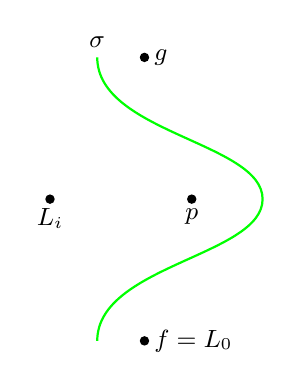
\begin{tikzpicture}[scale=0.6]
	\fill[black]
	(2,0) circle[radius=1mm]
	  node[right]{\small \(f = L_0\)}
	(0,3) circle[radius=1mm]
	  node[below]{\small \(L_i\)}
	(3,3) circle[radius=1mm]
	  node[below]{\small \(p\)}
	(2,6) circle[radius=1mm]
	  node[right]{\small \(g\)};
	\draw[thick,green] (1,6) .. controls (1,4.4) and (4.5,4.2) ..
	                   (4.5,3) .. controls (4.5,1.8) and (1,1.6) .. (1,0);
	\draw (1,6) node[above]{\small \(\sigma\)};
      \end{tikzpicture}
      \caption{ }
      \label{fig:entga}
   \end{subfigure}\hspace{0.4cm}
   \begin{subfigure}[t]{0.36\textwidth} \centering
      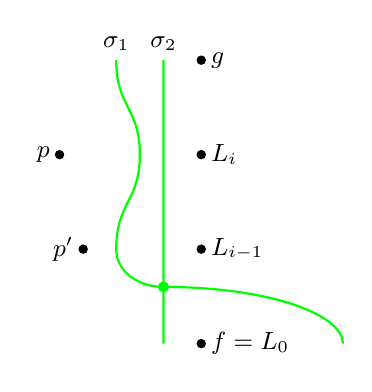
\begin{tikzpicture}[scale=0.6]
	\fill[black]
	(3,0) circle[radius=1mm]
	  node[right]{\small \(f = L_0\)}
	(3,2) circle[radius=1mm]
	  node[right]{\small \(L_{i-1}\)}
	(3,4) circle[radius=1mm]
	  node[right]{\small \(L_i\)}
	(3,6) circle[radius=1mm]
	  node[right]{\small \(g\)}
	(0.5,2) circle[radius=1mm]
	  node[left]{\small \(p^\prime\)}
	(0,4) circle[radius=1mm]
	  node[left]{\small \(p\)};
	\draw[thick,green] (2.2,0) -- (2.2,6)
	  (1.2,6) .. controls (1.2,5) and (1.7,5) ..
	  (1.7,4) .. controls (1.7,3) and (1.2,3) ..
	  (1.2,2) .. controls (1.2,1.5) and (1.7,1.2) ..
	  (2.2,1.2) node[circle,fill=green,inner sep=0.5mm]{ }
	  .. controls (4.5,1.2) and (6,0.6) .. (6,0);
	\draw (1.2,6) node[above]{\small \(\sigma_1\)}
	      (2.2,6) node[above]{\small \(\sigma_2\)};
      \end{tikzpicture}
      \caption{ }
      \label{fig:entgb}
   \end{subfigure}\hspace{0.4cm}
